% Electromagnetism

\documentclass[11pt]{article}

\usepackage[a4paper, margin=1in]{geometry}

\usepackage{amsmath}

\usepackage{amssymb}

\usepackage[german]{babel}

\usepackage[autostyle=true]{csquotes}

\usepackage{libertine}

\usepackage[libertine]{newtxmath}

\usepackage{tikz}

\usepackage{gensymb}

\usepackage{fancyhdr}

\usepackage{amsfonts}

\usepackage{pgfplots}

\pgfplotsset{compat=1.10}

\usepackage{multicol}

\usepackage{caption}

\usepackage{floatrow}

\everymath{\displaystyle}

% Header / footer settings

\pagestyle{fancy}
\fancyhf{}
\renewcommand{\headrulewidth}{0.2mm}
\fancyhead[C]{Funktionen}
\renewcommand{\footrulewidth}{0.2mm}
\fancyfoot[L]{Peter Goldsborough}
\fancyfoot[C]{\thepage}
\fancyfoot[R]{\today}

\fancypagestyle{plain}{%
	\fancyhf{}
	\renewcommand{\headrulewidth}{0mm}%
	\renewcommand{\footrulewidth}{0.2mm}%
	\fancyfoot[L]{Peter Goldsborough}
	\fancyfoot[C]{\thepage}
	\fancyfoot[R]{\today}
}


\setlength{\headheight}{15pt}

\setlength{\parindent}{0pt}

\addtolength{\parskip}{\baselineskip}


\newcommand{\overbar}[1]{\mkern 1.5mu\overline{\mkern-1.5mu#1\mkern-1.5mu}\mkern 1.5mu}

\newcommand{\heading}[1]{\begin{center}\Huge \textbf{#1}\end{center}\par}

\newcommand{\sub}[1]{\vspace{\parskip}{\LARGE\textbf{#1}}}

\newcommand{\subsub}[1]{{\Large \textbf{#1}}}

\newcommand{\subsubsub}[1]{\textbf{#1}}

\newcommand{\colvec}[1]{\begin{pmatrix}#1\end{pmatrix}}

\newcommand{\extrapar}{\par\vspace{\baselineskip}}

\newcommand{\zitat}[1]{\foreignquote{german}{#1}}

\newcommand{\bolditem}[1]{\item \textbf{#1}}

\newcommand{\titleitem}[1]{\bolditem{#1}\par}

\newcommand{\defas}{ \dots \,\,}

\begin{document}
\thispagestyle{plain}

\heading{Electromagnetism}

Similar to how there are two types of charges --- positive and negative --- there are also two types of magnetic poles: \emph{north} or \emph{south}. Like poles repel, while opposite poles attract. When current flows and charges move through a conductive material, a magnetic field is generated around it. Similarly, a magnetic field may produce a current under certain circumstances. 

The magnetic field produced by a current was first discovered by Hans Christian Oersted, a Danish physicist, in 1820. By accident, he had placed a magnetic needle next to a wire. When connecting the wire to a power supply and thus letting an electric current flow through it, he observed that the needle changed its direction. More precisely, he defined four possible cases:

\begin{enumerate}
	\item When \textbf{no current} was flowing, the needle aligns to the earth's magnetic field.

	\item When \textbf{current flows}, the needle moves out of it's original position

	\item When the \textbf{current direction is reversed}, the needle moves in the opposite direction relative to that of the second case.

	\item When the \textbf{current strength is increased}, the deflection of the needle increases.
\end{enumerate}

\sub{Magnetic Field around a Straight Wire}

The magnetic field created by an electric current flowing through a straight wire has a very characteristic shape: the magnetic field lines are structured in \emph{concentric circles} around the wire. This means that all field lines of the magnetic field move circularly around the wire (the center of their rotation), while each is spaced at a different distance or \emph{radius} to it. The shape of the resultant magnetic field can be found by laying out ferromagnetic material, such as iron filings, around the wire through which current is flowing.

\begin{plot}
	
	% Wire
	\draw [->]
	      (0, 0, 0) node [below] {$+$}
	   -- (0, 4, 0) node [above] {$-$}
	      node [pos=0.8, right] {$I$};

	% Circles
	\begin{scope}[canvas is zx plane at y=2]
		\foreach \r in {0.4, 0.8, ..., 2}
		{	
			\draw [->, red]
			      (\r, 0) arc [radius=\r, start angle=0, end angle=350];
		}
	\end{scope}

\end{plot}

The strength of the magnetic field decreases with its distance from the wire, as the circumference of the concenctric circles naturally increases with the radius (i.e. the magnetic field is spread out to a greater extent). This leads to the following definition for the magnitude or \emph{strength} of the magnetic field $B$ at any distance $r$ from the wire: $$B = \frac{\mu_0 \cdot I}{2 \pi \cdot r}$$

\pagebreak

In the above equation $\mu_0$ is a constant value signifying the permittivity of free space (vacuum and air), while $I$ is the strength of the current flowing through the wire. As can be determined from this equation, the magnetic field is directly proportional to the rate at which charges flow through the conductor, meaning $B$ generally increases with any increase in current. Additionally, it can be seen that the strength of the magnetic field is inversely proportional to the distance $r$ and essentially the circumference $2\pi \cdot r$ of the concenctric circle. When attempting to determine the direction of the magnetic field produced, one may apply the so-called \emph{right-hand-grip rule}. For this, the thumb of your right hand should point in the direction in which current is flowing (technical current direction, from plus to minus). The direction of the magnetic field lines is then that in which the fingers of your right hand curl.

\sub{Magnetic Field in and around a Solenoid}

A \emph{solenoid} is a tightly wound coil of wire. When carrying current, it also produces a magnetic field with a very characteristic shape and structure. Outside the solenoid, i.e. around the coiled region of the wire, the magnetic field is simlar in shape to a bar magnet and its strength decreases with increasing distance, as was the case for a straight wire. Inside the solenoid, however, the field lines are parallel with a constant density and field strength. The magnetic field inside a solenoid is therefore referred to as a \emph{homogenous field} --- it is uniform in strength and density.

\begin{plot}

	% Coil
	\foreach \i in {0, 0.5, ..., 4}
	{
		\begin{scope}[canvas is zx plane at y=\i]

			\draw [->] (0, 0) arc (10:360:1);

		\end{scope}
	}

	\foreach \a/\b/\c/\d/\e in {0.1/7/3/1/-2,
								0.2/6.5/2.5/1/-1.5,
							    0.4/6/2/1/-1,
							    0.6/5.5/1.5/1/-0.5}
	{
		% First side
		\draw [red, ->]
	      (\a, 0, 0) -- +(0, 4.5, 0)
	      .. controls (\d, \b) and (\c, 4) .. (\c, 2.2);

	    \draw [red] (\c, 2) .. controls (\c, 0) and (\d, \e) .. (\a, 0); 

	    % Second side
	    \draw [red, ->]
	      (-\a, 0, 0) -- +(0, 4.5, 0)
	      .. controls (-\d, \b) and (-\c, 4) .. (-\c, 2.2);

	    \draw [red] (-\c, 2) .. controls (-\c, 0) and (-\d, \e) .. (-\a, 0); 
	}


	 % North
	 \draw (0, 5.7, 0) node {\Large N};

	 % South
	 \draw (0, -1.3, 0) node {\Large S};

\end{plot}

The overall strength of the magnetic field $B$ inside the core of the solenoid is dependent on three factors. The first is again the strength $I$ of the current flowing through the solenoid, to which the magnetic field strength $B$ is directly proportional. The second variable is the number of turns of the coil $N$. The greater the number of turns, the greater is the field strength --- again a direct proportionality. Lastly, the magnetic field strength $B$ is inversely proportional to the length $l$ of the solenoid. The reason why is that given a constant number of turns $N$, a decrease in the length would mean that the turns are packed more tightly, while increasing the length would loosen the winding of the solenoid. These factors lead to the following relationship and equation to calculate the magnetic field strength $B$ inside the core, where the magnetic field is homogenous and thus uniform with this strength: $$B = \mu_0 \cdot \frac{N \cdot I}{l}$$ Often, the number of turns divided by the length of the solenoid is reduced to a constant $n$, where $n$ is then the number of turns per unit length. Another thing to mention is that the strength of the field can be increased by inserting an iron core into the solenoid. This is the result of the ferromagnetic properties of iron, which may cause an increase in field strength by several orders of magnitude.

When trying to determine which side of the solenoid --- which acts as a magnet --- is the north pole, the region which, by convention, is defined as the source of the magnetic field lines, and which the south pole, one may use a different form of right-hand rule: the \emph{right-hand rule for solenoids}. In this case, place your \emph{right} hand around the solenoid, such that your fingers curl in the same way in which the current is circularly flowing through the windings of the coil. The north pole is then on the side of your thumb, meaning the magnetic field lines point in the opposite direction of your thumb.

\sub{The Lorentz Force}

The Lorentz force $\vec{F}$ is the force exerted on a moving electric charge of magnitude $q$ with velocity $\vec{v}$, by the combination of a magnetic field $\vec{B}$ and an electric field $\vec{E}$. The direction of the Lorentz force is always perpendicular to the electric field $\vec{E}$ and corresponding current, as well as to the magnetic field $\vec{B}$. Therefore, the Lorentz force acting on a charged particle is mathematically defined as the cross product of the magnetic field $\vec{B}$ and $q \cdot \vec{v}$, the product of the magnitude of the charge and its velocity: $$\vec{F} = q \cdot \vec{v} \times \vec{B}$$ The direction of deflection of the moving charges is thus dependent on the current direction and the magnetic field direction. The strength of the Lorentz force, on the other hand, depends on the strength of the current $I$ flowing through the wire as well as on the strength of the magnetic field $\vec{B}$ through which the charges pass.

\begin{plot}

	% Magnetic field
	\draw [->, blue]
	      (0, 0, 0) -- (0, 0, 2.5) node [midway, above, right] {$\vec{B}$};

	% Charge
	\draw [fill=black] (0, 0, 0) circle [radius=2pt] node [right] {$q$};

	% Velocity (electric field)
	\draw [->, red]
	      (0, 0, 0) -- (-2, 0, 0) node [midway, above] {$\vec{v}$};

	% Lorentz force
	\draw [->]
	      (0, 0, 0) -- (0, 2, 0) node [midway, right] {$\vec{F}$};


\end{plot}

An example of the Lorentz force in action is when a single loop of wire is placed in the magnetic field of a horseshoe magnet. When direct current flows through the wire, the Lorentz force will deflect the wire in a direction that is perpendicular to both the electric field --- i.e. the current, from the positive to the negative pole --- as well as the magnetic field, which flows from the north to the south pole of the horseshoe magnet. This direction must be \emph{inwards}, into the horseshoe magnet. One method of determining the direction in which the Lorentz force acts is the \emph{right-hand rule for the Lorentz force}. For this, the fingers of one's open hand should point from north to south pole, i.e. towards the south pole. Next, one must turn one's right hand is such a way that one's thumb points into the technical current direction, from plus to minus. The direction of the Lorentz force acting on the moving charged particles of the wire is subsequently the direction in which one's right hand now pushes, perpendicular to the open palm. It is important to note that if the current direction $\vec{v}$ is parallel to the magnetic field direction $\vec{B}$, the Lorentz force does not act.

\pagebreak

\sub{Deflection of Electron or Ion Beams}

\subsub{Electric Fields}

When a charged particle moves through an electric field created by a positively and negatively charged plate, the particle is deflected towards the plate whose charge is opposite to that of the moving particle. Which one depends on the charge of the particle. If the particle is positively charged, as is the case for, say, a \emph{proton}, it is deflected towards the negative plate. If the charge is however negative, as is an electron, it is again deflected towards the plate of opposite charge, thus now the positive plate. The force with which this charged particle is deflected can be determined by multiplying the magnitude of the moving charge with the electric field vector $\vec{E}$, as the latter value is a measure of the electrostatic force exerted within the electric field on one unit charge.

\begin{plot}
	
	% Positive plate
	\draw (0, 2) -- +(4, 0);

	% Negative plate
	\draw (0, 0) -- +(4, 0);

	% Positive and negative charges on plates
	\foreach \x in {0, 0.5, ..., 4}
	{
		\draw [red] (\x, 2.5) node {$+$};

		\draw [blue] (\x, -0.5) node {$-$};
	}

	% Positive moving charge path
	\draw [dashed, red] (-1, 1) .. controls (0.5, 1) .. (2, 0);

	% Positive charge
	\draw [red] (0.7, 1.2) circle [radius=0.2cm] node {$+$};

	% Positive moving charge path
	\draw [dashed, blue] (5, 1) .. controls (3.5, 1) .. (2, 2);

	% Positive charge
	\draw [blue] (3.3, 0.8) circle [radius=0.2cm] node {$-$};

	% Equation
	\draw (7, 1) node {$\vec{F} = q \cdot \vec{E}$};

\end{plot}

\subsub{Magnetic Fields}

When charged particles enter a magnetic field, the Lorentz force acts on them, as the Lorentz force is the force exerted upon a moving charge in a magnetic field. This is, of course, only the case if the magnetic field and electric field (current) direction are not parallel, but perpendicular to each other. When a charged particle moves through a magnetic field that is perpendicular to it and points into the plane, the Lorentz force will cause the charge to move along a circular path. More precisely, the Lorentz force acts as the centripetal, \emph{center-seeking}, force, that continuously causes the charged particle to deflect from its tangential, inertial path and accelerate towards the center of its rotational motion. This is the result of the Lorentz force acting perpendicular to the tangent in every point of the charge's circular motion. Given this information, the radius of the charges's motion can be determined by equating the formula for the centripetal force $F_c$ with the Lorentz force $F_m$ equation. Note that the magnitude of the velocity and magnetic field vectors are used, turning the cross product into a normal (scalar) multiplication: $$F_c = F_m \thus m \cdot \frac{v^2}{r} = q \cdot v \cdot B \thus r = \frac{m \cdot v}{q \cdot B}$$

\begin{plot}
	
	% Magnetic fiel pointing into plane
	\foreach \row in {0, ..., 3}
	{
		\foreach \column in {0, ..., 3}
		{
			\draw (\row, \column) circle [radius=0.3cm] node {$\times$};
		}
	}

	% Magnetic field label
	\draw (1.5, -1) node {Magnetic field $\vec{B}$ pointing into plane};

	% Charge arriving path
	\draw [dashed, blue] (-2.5, 3) -- (0, 3);

	% Charge arriving
	\draw [blue] (-2.8, 3) circle [radius=0.2cm] node {$-$};

	% Circular path of charge
	\draw [dashed, blue] (0, 1.5) circle [radius=1.5cm];

	% Charge in orbit
	\draw [blue] (-1.7, 1.5) circle [radius=0.2cm] node {$-$};

	% Force acting (centripetal and Lorentz)
	\draw [->] (-1.5, 1.5) -- +(1.2, 0)
	      node [above, midway] {$\vec{F_c}$};

\end{plot}

\pagebreak

\sub{Applications of Electromagnetism}

\subsub{The Relay}

One application of the principles of electromagnetism just mentioned is a \emph{relay} (often written as \emph{relais}). A relay is a special type of circuit consisting of two contacts, a ferromagnetic switch and a solenoid. One of the two contacts is normally connected to the ferromagnetic switch and is thus referred to as the \emph{Normally-Closed (NC)} contact. The other contact is normally open and is appropriately called the \emph{Normally-Open (NO)} contact. The interesting property of a relay circuit is that when current is allowed to flow through the relay and so that it consequently produces a magnetic field, the ferromagnetic switch is attracted by the generated field. As a result, the switch is pulled towards the normally open contact and thus closes the NO-circuit, while opening the NC circuit. Once the current flowing through the solenoid is interrupted, its magnetic field fades. A spring system thereafter ensures that the switch springs back to its usual position, closing the normally-closed circuit. One possible, actually useful electric circuit utilizing a relay is given below.

\begin{circuit}
	
	% Circuit
	\draw (1, 0) to [battery] (0, 0) -- ++(0, -2)
	      to [push button] ++(5, 0)
	 -- ++(0, 0.5)
	      to [cute inductor] ++(2, 0)
	 -- ++(0, -0.5) -- ++(0.5, 0)
	 -- ++(0, 4) -- ++(-5, 0) -- ++(0, -1)
	      to [lamp] ++(3, 0)
	 -- ++(0.5, 0) arc (0:-180:0.2) node [right] {\hspace{0.4cm} NC}
	    ++(-3.1, 0) -- ++(0, -1.5)
	    to [lamp] ++(3, 0)
	 -- ++(0.5, 0) arc (0:180:0.2) node [right] {\hspace{0.4cm} NO}
        ++(-3.1, 0) ++(0, 0.5) -- (1, 0);

    % Feromagnetic switch
    \draw (0, -1) -- ++(3, 0) -- ++(0, 1.3) -- ++(2, 0) -- +(28:1);

\end{circuit}

\subsub{The Solenoid Lock}

Another common use of solenoids and electromagnetism in the household is a \emph{solenoid lock}, usually used for electronically locked doors. The basic principle of such a lock involves a feromagnetic bolt that is placed inside a solenoid, with a spring between the bolt and the back of the casing of the lock. Moreover, the solenoid must be connected to some form of power supply and there should exist a switch or button to let current flow through the solenoid or not. When no current flows so that no magnetic field is generated, the bolt sticks out of the casing of the lock and usually into the door that it is supposed to keep shut. The spring behind the bolt is responsible for this. However, once the solenoid is switched into the circuit and current flows through it, it generates a magnetic field inside its core and around it. The bolt is situated in its core, so it will come into the influence of the homgenous magnetic field of uniform density and strength that is characteristic of solenoid cores. Given that the coil is wound in the right direction, i.e. in a way that so that the south pole is on the side of the door and the north pole at the back of the casing (the magnetic flux direction is from south to north \emph{inside the core}), the magnetic field produced will cause the bolt to move backwards, out of the door to unlock it. Once the current stops flowing, the spring ensures that the natural position of the bolt, locking the door, is restored.

\begin{plot}
	
	% Door
	\draw (0, -1.25) -- ++(0, 1.25) ++(0, 0.75) -- ++(0, 1.25);

	% Bolt
	\draw (-0.5, 0.65)
	 -- ++(3, 0)
	 -- ++(0, -0.5)
	 -- ++(-3, 0)
	 -- ++(0, 0.5);

	% Solenoid, top
	\draw (0, 0.75) -- ++(5, 0) -- ++(0, 0.5) -- ++(-5, 0);

	% Coils out of plane
	\foreach \i in {1, 2, 3, 4}
	{
		\draw (\i, 1) circle [radius=0.2cm];
		\draw [fill=black] (\i, 1) circle [radius=1.2pt];
	}

	% Back
	\draw (5, 0.75) -- ++(0, -0.75) -- ++(-0.5, 0) -- ++(0, 0.75);

	% Solenoid, bottom
	\draw (0, 0) -- ++(5, 0) -- ++(0, -0.5) -- ++(-5, 0);

	% Coils into plane
	\foreach \i in {1, 2, 3, 4}
	{
		\draw (\i, -0.25) circle [radius=0.2cm] node {$\times$};
	}

	% Spring
	\foreach \i in {2.8, 2.9, ..., 4.2}
	{
		\draw (\i, 0.375) circle [radius=0.3cm];
	}

\end{plot}

\pagebreak

\subsub{The Cathode Ray Tube}

For a long time, before LCD, LED or Plasma screens became the standard for television screens or computer monitors, \emph{cathode ray tubes} were used to project images onto phosphorescent screens. Cathode ray tubes consist of five main components, listed below.

\begin{itemize}

	\titleitem{Heated Cathode}

	The first and most important component of a cathode ray tube is, as the name suggests, a cathode. The cathode is a negatively charged metal plate warmed by a heating system and kept at a negative potential. The energy supplied to the electrons is enough for the negatively charged particles to escape from the heated cathode as to interact with the other components of the cathode ray tube. To ensure that a constant beam of electrons leaves the cathode, new electrons are continuously supplied by the negative terminal of the power supply to which the cathode is connected.

	\titleitem{Wehnelt grid}

	After electrons escape from the heated cathode by virtue of the thermal energy supplied to them, they subsequently interact with what is referred to as a \emph{Wehnelt grid} or \emph{cylinder}. Such a Wehnelt grid is essentially an electrode with an electric potential that is slightly more negative than that of the cathode. As a consequence, when the electron ray coming from the heated cathode comes near this grid, some electrons with sufficient energy and velocity will be able to overcome the electrostatic force of repulsion exerted from the Wehnelt grid on the electrons and are able to travel through an opening in it. However, other negatively charged particles may not have been supplied with enough energy to overcome the Wehnelt grid and will be repelled by it. The purpose of the Wehnelt grid is to act as a mechanism for controlling the number of electrons able to pass through the cathode ray tube. Ultimately, this makes it possible to control and adjust the brightness of the screen.

	\titleitem{Anode}

	The anode is a positively charged metal plate with an opening at its center. It is used to accelerate the electrons via an electrostatic force of attraction and also has the role of focusing the electron ray as much as possible.

	\titleitem{Magnetic Deflection System}

	After passing through the anode, the electrons subsequently interact with an array of solenoid coils. Two such coils are placed above and below the path of the electrons, while two are placed to their right and left. A certain variable electric current flowing through the solenoids generates a seperate magnetic field in each coil as well as between two directional pairs (vertical or horizontal). Depending on the strength of the current flowing through them and the resultant magnetic field created, the principles of the Lorentz force --- the force acting on moving electrical charges in an magnetic field --- cause the electrons to be deflected in a certain way. The coils to the right and left of the elctrons are responsible for the vertical deflection of the electron ray, while the strength of the magnetic field between the solenoids above and below the electrom beam determine its horizontal direction. This inverse relationship is due to the nature of the Lorentz force, which acts perpendicular to both the magnetic field direction and to the current direction. By varying the vertical and horizontal magnetic field strength the degree of deflection in both the y and the x plane can be controlled. This is ultimately how each point on the screen can be adressed.

\pagebreak

	\titleitem{Phosphorescent Screen}

	The last and final stop of the electron beam is the phosphorescent screen at the end of the cathode ray tube. When electrons hit the screen covered with phosphorescent material, their kinetic energy causes the screen to glow. To prevent the screen from becoming negatively charged, it is additionally covered with graphite to direct the electrons to ground. If this were not done, the increasingly negatively charged screen would eventually cause electrons to be repelled, thereby reducing the brightness of the picture produced.

\end{itemize}

\begin{plot}
	
	% Tube outline
	\draw (0, 2) -- ++(5, 0)
	 -- ++(20:6) .. controls +(0.5, -3.05) .. ++(0, -6.1) -- ++(160:6)
	 -- (0, 0) -- (0, 2);

	% Cathode
	\draw (0, 0.8) -- ++(1, 0) -- ++(0, 0.4) -- ++(-1, 0);

	\draw [->] (-0.8, 1) node [left] {Cathode} -- ++(1.3, 0);

	% Wehnelt grid
	\draw (0, 0.5) -- ++(1, 0)
	   arc (-90:-25:0.5) ++(0, 0.4) arc (25:90:0.5)
	-- ++(-1, 0);

	\draw [->] (0.5, 2.5) node [above] {Wehnelt Grid} -- ++(0, -0.9);

	% Anode
	\draw (2, 0.2) -- ++(0.2, 0)
	 -- ++(0, 0.5) ++(0, 0.5)
	 -- ++(0, 0.5) -- ++(-0.2, 0);

	 \draw [->] (1.5, -0.7) node [below] {Anode} -- ++(70:1);

	% Magnetic deflection mechanism, top
	\draw (2.8, 2.1) -- ++(1.8, 0)
	 -- ++(0, 0.6) -- ++(-1.8, 0)
	  -- ++(0, -0.6);

	% Magnetic deflection mechanism, bottom
	\draw (2.8, -0.1) -- ++(1.8, 0)
	 -- ++(0, -0.6) -- ++(-1.8, 0)
	 -- ++(0, 0.6);

	\draw [->]
	      (3.5, 3.5) node [above] {Magnetic Deflection System}
	   -- ++(0, -0.7);

	% Electron ray
	\draw [dashed, very thick, blue]
	      (1, 1) -- ++(4, 0) .. controls ++(3, 0) .. ++(6, 1);

    % Light
    \foreach \a/\c in {60/red, 30/orange, 0/yellow, -30/green, -60/blue}
    {
    	\draw [\c] (11, 2) -- ++(\a:0.6);
    }

	% Phosphorescent screen label
	\draw [->] (7, -2) node [below] {Phosphorescent Screen} -- ++(30:4.2);

\end{plot}

\subsub{The Electric Motor}

To discuss the next application of electromagnetism presented here, it must first be investigated how a force acts on a wire of length $l$ in a magnetic field of strength and direction $\vec{B}$, where the direction of $\vec{B}$ is perpendicular to the direction in which the current $I$ flows. In this case, the Lorentz force --- the force exerted on moving charges in a magnetic field --- acts perpendicular to both the magnetic field and the flow of charges. In the below representation, this would cause the wire to move inwards, into the plane.

\begin{plot}

	% Wire
	\draw (0, 0) -- ++(10, 0) -- ++(0, 1) -- ++(-10, 0) -- ++(0, -1);

	% Charges
	\foreach \i in {0.5, 2.5, ..., 8.5}
	{
		\draw [blue] (\i, 0.4) circle [radius=0.2cm] node {$-$};

		\draw [blue] (\i + 1, 0.6) circle [radius=0.2cm] node {$-$};
	}

	% Terminals
	\draw (-1, 0.5) node {\Large $+$};
	\draw (11, 0.5) node {\Large $-$};

	% Current direction
	\draw [->] (3, 1.5) -- (7, 1.5) node [midway, above] {$I$};

	% Length of wire
	\draw [<->] (0, -0.5) -- (10, -0.5) node [midway, below] {$l$};

	% Magnetic field lines
	\foreach \i in {1, ..., 9}
	{
		\draw [->, red] (\i, 1.3) -- ++(0, -1.6);
	}

	% Magnetic field label
	\draw [red] (9, 1.8) node {$\vec{B}$};

\end{plot}

Interestingly, there exists a relationship of direct proportionality between the current $I$, the length of the wire $l$ and the magnetic field $\vec{B}$. To come to this conclusion, one must first consider that current $I$ is defined as the rate at which charges flow through a certain point of a circuit, thus as the magnitude of the charge $q$ divided by the time taken $t$. Moreover, one should remember the definition of the Lorentz force $F$ as the cross product between the magnetic field and the product of the size of the charge $q$ and its velocity vector $\vec{v}$. Lastly, it must be mentioned that when the magnetic field direction and the current direction are perpendicular to each other, the cross product of the Lorentz force becomes a dot (scalar) product. $$I = \frac{q}{t} \hspace{1cm} F = q \cdot \vec{v} \times \vec{B} \hspace{0.5cm} \xrightarrow{\text{if } \vec{B} \, \perp \, \vec{v}} \hspace{0.5cm} \vec{F} = q \cdot \vec{v} \cdot \vec{B}$$ 

\pagebreak

In the next step, the current equation must be solved for the charge. Also, the time taken by the charge can be replaced by the length of the wire divided by the velocity of the charges (from the definition of velocity as displacement over time). $$I = \frac{q}{t} \AND t = \frac{l}{v} \thus q = I \cdot t = I \cdot \frac{l}{v}$$ Now, this expression of charge being equal to the current multiplied by the length and divided by the velocity can be substituted for the charge of the Lorentz force equation, yielding an expression that makes the Lorentz force $\vec{F}$ depend directly on the current $I$, the length of the wire $l$ and the magnetic field strength $\vec{B}$: $$\vec{F} = q \cdot \vec{v} \cdot \vec{B} = I \cdot \frac{l}{v} \cdot \vec{v} \cdot \vec{B} \thus \vec{F} = I \cdot l \cdot \vec{B}$$

Now, it can be discussed how a single loop of wire acts in a magnetic field. There are two possible scenarios for this. In the first case, the loop of wire is perpendicular to the magnetic field. In the second scenario, the single loop of wire is no longer perpendicular to the magnetic field, but is now at some angle other than $90\degree$ relative to it. Both cases and their implications are discussed below.

\subsubsub{Loop of Wire $\perp \vec{B}$}

When the magnetic field and the loop of wire are perpendicular to one another, the Lorentz force exerted on the moving charges within the wire are pushed in the outward direction at every point in the circuit. As a result, any Lorentz force $\vec{F_1}$ acting on electrons on one side of the loop is balanced out by the Lorentz force $\vec{F_2}$ acting on the opposite end of the wire, as the first force $\vec{F_1}$ will be equal in magnitude but opposite in direction compared to the second force $\vec{F_2}$, such that $\vec{F_1} = -\vec{F_2}$ and $|\vec{F_1}| = |\vec{F_2}|$. The net force acting on the single loop of wire is therefore zero. Thus it can be said that if the loop of wire and the magnetic field $\vec{B}$ are perfectly perpendicular to each other, the loop of wire will not move, but stay at rest.

\begin{plot}

	% Loop of wire
	\begin{scope}[canvas is zx plane at y=0]

		\draw [thick, -<] (0, 0) -- ++(1, 0);

		\draw [thick, -<] (1, 0) -- ++(1, 0) -- ++(0, -0.9);

		\draw [thick, -<] (2, -0.9) -- ++(0, -0.9) -- ++(2, 0);

		\draw [thick, -<] (4, -1.8) -- ++(2, 0) -- ++(0, 2) node [below] {$I$};

		\draw [thick, -<] (6, 0.2) -- ++(0, 2) -- ++(-2, 0);

		\draw [thick, -<] (4, 2.2) -- ++(-2, 0) -- ++(0, -0.9);

		\draw [thick, -<] (2, 1.3) -- ++(0, -0.9) -- ++(-2, 0);

	\end{scope}

	% Force 1
	\draw [->] (-1.8, 0, 5) -- ++(-2, 0, 0)
		       node [pos=0.7, above] {$\vec{F_1}$};
 
    % Force 2
	\draw [->] (2.2, 0, 5) -- ++(2, 0, 0)
		       node [pos=0.7, above] {$\vec{F_2}$};

    % Magnetic field lines
    \foreach \i in {-2, -1, ..., 2}
    {
    	\foreach \j in {1, 2, ..., 4}
    	{
    		\begin{scope}[canvas is xy plane at z=\j]

    			\draw [red, ->] (\i, 1) -- ++(0, -3);

    		\end{scope}
    	}
    }

    % Magnetic field label
    \draw [red] (-0.5, 1.5, 1) node {$\vec{B}$};

\end{plot}

\subsubsub{Loop of Wire not $\perp \vec{B}$}

In the second scenario, the single loop of wire is no longer perpendicular to the magnetic field. Therefore, it is no longer the case that any force acting on electrons on one side of the loop is cancelled by an equal and opposite force on the other end of the loop. Rather, the Lorentz force exerted on charged particles on the first side will be \emph{parallel} to the force acting on the wire on the opposite side, but \emph{not identical}. Thus, as one force at a position higher in the magnetic field pulls the wire in one direction and as another force on the opposing side, at a position that is lower in the magnetic field, pulls in the opposite direction, a \emph{torque} (a force causing rotation) is created and the loop will begin to rotate. This is the result of the charged particles' and loop's inertia --- their resistance to change their state of motion, as the Lorentz force supplies both sides of the loop of wire with a certain linear momentum. When the higher up point commences its forward motion it will attempt to do so as long as possible. The only way to continue the forward motion is for the loop to move downward (this prolongs the forward motion). At the lower point, the same principle of inertia and linear momentum applies and the loop will this time attempt to move upward to resist changes to its state of motion as long as possible. As a side note: any two forces acting on the loop and interacting in the manner just described are referred to as \emph{force couples}. In any case, once the loop of wire is rotating, it is given angular momentum. When the loop's rotational motion progresses to such an extent that it is again in a position perpendicular to the magnetic field, it is the angular momentum and inertia that does not cause the loop to stop, but continue, even though the force couple balances itself at this position. One last thought to mention is that if the angular momentum of the loop resulting from the Lorentz force acting on the force couple is not great enough, the loop of wire might not be able to achieve a full rotation (even after crossing the perpendicular position just described). Consequently, the loop will oscillate up and down as each side of the loop oscillates between one position higher and one lower in the magnetic field, where the Lorentz force pulls the loop back to the respective previous position. The initial impulse supplied by the Lorentz force, in dependence of the current $I$, the length of the wire $l$ and the magnetic field $\vec{B}$, must therefore be great enough to overcome this threshold.

\begin{plot}

	% Loop of wire
	\begin{scope}[canvas is zx plane at y=0]

		\draw [thick, -<] (0, 0) -- ++(1, 0);

		\draw [thick, -<] (1, 0) -- ++(1, 0) -- ++(0, -0.9);

		\draw [thick, -<] (2, -0.9) -- ++(0, -0.9) -- ++(2, 0);

		\draw [thick, -<] (4, -1.8) -- ++(2, 0) -- ++(0, 2) node [below] {$I$};

		\draw [thick, -<] (6, 0.2) -- ++(0, 2) -- ++(-2, 0);

		\draw [thick, -<] (4, 2.2) -- ++(-2, 0) -- ++(0, -0.9);

		\draw [thick, -<] (2, 1.3) -- ++(0, -0.9) -- ++(-2, 0);

	\end{scope}

	% Force 1
	\draw [->] (-1.8, 0, 5) -- ++(-2, 0, 0)
		       node [pos=0.7, above] {$\vec{F_1}$};
 
    % Force 2
	\draw [->] (2.2, 0, 5) -- ++(2, 0, 0)
		       node [pos=0.7, above] {$\vec{F_2}$};

    % Magnetic field lines
    \foreach \i in {-2, -1, ..., 2}
    {
    	\foreach \j in {1, 2, ..., 4}
    	{
    		\begin{scope}[canvas is xy plane at z=\j, rotate=20]

    			\draw [red, ->] (\i, 1) -- ++(0, -3);

    		\end{scope}
    	}
    }

    % Magnetic field label
    \draw [red] (-0.5, 1.5, 1) node {$\vec{B}$};

\end{plot}

\subsub{The DC Electric Motor}

A practical direct current (DC) electric motor uses a different principle than that of the aforementioned electric motor. It consists of the following components:

\begin{itemize}
	
	\item A \textbf{permanent magnet} to create a constant magnetic field. The magnet is referred to as a \emph{stator}, because it is stationary. It has a constant and predefined north and south pole.

	\item One or more \textbf{rotating coils}. These coils are called the \emph{rotor} part of the motor, because they are rotating. When current flows through such a coil (solenoid), it generates a magnetic field similar to that of a bar magnet, with a north and south pole. Which side is north and which south depends on the direction in which the current is flowing through the coil. The basic principle of the motor is then to let current flow through two coil pairs on either side of the motor in such a way, that the coil on the north side of the permanent magnet has its magnetic north on top while the coil on the other side of the magnet --- where the stator's south pole is --- has its south pole on top. As a consequence, each coil is repelled as much as possible. The strength of the repulsion depends on the strength of the magnetic field $\vec{B}$ generated by the coil, which is defined as $\vec{B} = \mu_0 \cdot \frac{N}{l} \cdot I$. Of course, if the current direction were constant in each coil, the rotational motion could only work well for one half of a rotation. At that point, the north pole of the one coil would be aligned with the south pole of the stator and the other coil with the south pole on top would be perfectly aligned with the north pole. The attraction between the stator and rotor is such that the torque (the force responsible for rotation) is zero in this position. This may not necessarily lead to a standstill of the rotor, given its angular momentum and inertia, but would definitely hinder fluid motion. This problem is adressed by the next component. One more thought to add is that if the configuration of coils consists of two or of three coils, the rotor must be given an initial impulse to start rotating, as the magnetic forces are initially balanced (this is why real-world DC motors consist of many coils, then this problem is not present).

	\item A \textbf{commutator}, also referred to as a \emph{split ring}, which is fixed to the rotating coil. Such a commutator has several gaps in its conductive coating, such that when it is in contact with a power supply the current direction is reversed periodically. How often depends on the structure of the coil system. If, for example, two coils are used (i.e. two long, tightly wound loops of wire) there will be two gaps (or splits) in the commutator, such that the current direction is reversed every half turn. For a two-coil configuration, the result of this is that at the point of zero torque, in horizontal alignment with the stator, the current direction is reversed and thus also the polarity of the coils' magnetic fields. The coil which had north on top will now have south on top, just at the right moment for it to be repelled by the south pole of the stator.

	\item Graphite or carbon \textbf{brushes} that supply the \emph{direct} current to the commutator and thus to the coils. They are in physical contact with the split ring. These brushes are fixed, while the commutator rotates together with the coils.

\end{itemize} 

\begin{figure}[h!]
	\centering
	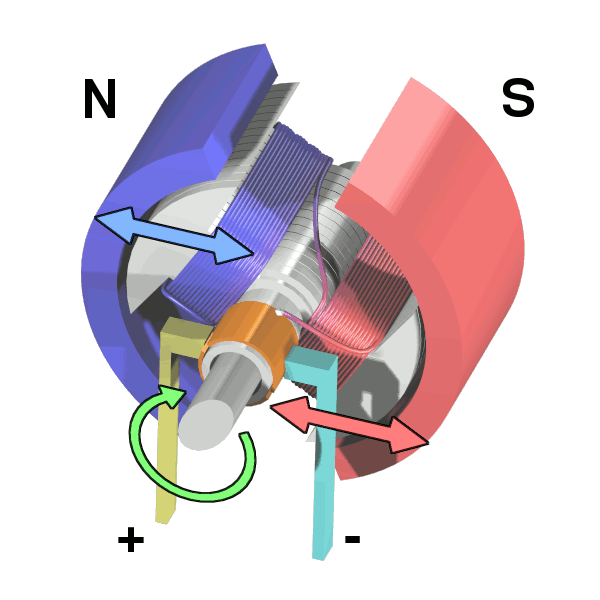
\includegraphics[scale=0.5]{img/motor.png}
	\caption{A DC Electric Motor}
\end{figure}

\pagebreak

\sub{Electromagnetic Induction}

Electromagnetic induction is the process by which a conductor placed in an alternating magnetic field or a conductor moving through a stationary magnetic field causes a voltage (potential difference) to be produced across the conductor. This process of electromagnetic induction, in turn, causes an electrical current --- it is said to \emph{induce} the current. In either case, the underlying, fundamental root of the generation of an induced electrical voltage is a certain change in \emph{magnetic flux}. Magnetic flux $\Phi_m$ is a measure of the amount of magnetic field passing through a given surface, i.e. that of the conductor, in case of electromagnetic induction. More precisely, it is mathematically defined as the magnetic field vector $\vec{B}$ multiplied by the perpendicular area $\vec{A}$ of the electric field that it penetrates. The vector $\vec{A}$ is the normal vector of the electric field plane, meaning that the length of $\vec{A}$, $|\vec{A}|$, yields the area of the electric field. Moreover, it should be mentioned that the product of any two vectors $\vec{a}$ and $\vec{b}$ can be replaced by the multiplication of their respective lengths, $|\vec{a}|$ and $|\vec{b}|$, as well as, additionally, the cosine of the angle $\alpha$ between the two vectors. This is a result of the definition of the formula for the cosine of the angle $\alpha$ between any two given vectors. All of these pieces of information put together yield the following definition for the magnetic flux $\Phi_m$ in dependence of the magnetic field $\vec{B}$ and the area vector $\vec{A}$: $$\Phi_m = \vec{B} \cdot \vec{A} \AND \cos \alpha = \frac{\vec{a} \cdot \vec{b}}{|\vec{a}| \cdot |\vec{b}|} \thus \Phi_m = |\vec{B}| \cdot |\vec{A}| \cdot \cos \alpha$$ The SI-unit of magnetic flux is Weber $[Wb]$, where one Weber is equivalent to one volt-second. The electrical voltage $U_{ind}$ induced from a given change in magnetic flux may subsequently be calculated as the difference in magnetic flux $\Delta \Phi_m$ divided by the difference in time or time taken $\Delta t$: $$U_{ind} = \frac{\Delta \Phi_m}{\Delta t}$$ This definition, referred to as \emph{Faraday's law of induction}, therefore makes clear that the voltage induced by an alternating magnetic field is equal to the rate of change of magnetic flux. However, there is one fault in the definition just given: the induced voltage is the \emph{negative} of the change of magnetic flux over time. The reason for this is given by \emph{Lenz' law}, which reads:

\begin{displayquote}

	The direction of the induced voltage is such, that if an induced current were able to flow, it would oppose the change that caused it.

\end{displayquote}

Essentially, this law, based on the law of energy conservation, states that the polarity of the induced voltage will be such that it produces a current whose \emph{magnetic field} opposes the change which produced it. The induced magnetic field inside any loop of wire always acts to keep the magnetic flux in the loop \emph{constant}. This means that if the voltage was induced as the result of the magnetic flux increasing, i.e. of $\vec{B}$ becoming greater, then the magnetic field of the induced current acts in opposition to it. If $\vec{B}$ is decreasing, the induced current's field acts in the direction that stops this decrease in order to (attempt to) keep the magnetic field constant. Thus, the correct definition of Faraday's law of induction is really (note the minus sign): $$U_{ind} = - \frac{\Delta \Phi_m}{\Delta t}$$

\pagebreak

\subsub{The AC-Generator}

Alternating current (AC) is a form of current that periodically changes its sign, thus its direction, from positive to negative and vice-versa, following a sinusoidal pattern. Conversely, direct current (DC) is unidirectional. Alternating current is the predominant form of current used in households. It is generated in power plants, where some source of energy, e.g. hydraulic power or wind power or nuclear fission power, transfers kinetic energy to turbines, which in turn operate the AC generator, which in turn generates electrical energy to power household or other appliances. The simplest setup of an AC-generator involves a stationary, permanent magnet with its north and south pole spaced apart, such that a magnetic field $\vec{B}$ is present. Between the poles one loop of wire is placed, which must be brought into rotational motion by some form of mechanical energy. Both ends of the loop of wire are connected to \emph{slip rings}, such that each end only touches one slip ring and the always the same slip ring for the whole duration of its rotation. Conductive carbon brushes connected to the slip rings make it possible to direct any induced current passing through the loop of wire to other locations, for other purposes. 

\begin{plot}
	
	% Loop of wire
	\begin{scope}[canvas is zx plane at y=0.5]

		\draw [thick]
			  (9, 0)
		 -- ++(-3, 0)
		 -- ++(0, -2)
		 -- ++(-5, 0)
	     -- ++(0, 4)
	     -- ++(5, 0)
         -- ++(0, -1.5)
         -- ++(3, 0);

	\end{scope}

	% North pole of magnet
	\draw (-4, 0, 7)
	 -- ++(-1, 0, 0) -- ++(0, 1, 0) ++(0, -1, 0)
	 -- ++(0, 0, -8) -- ++(0, 1, 0) ++(0, -1, 0)
	 -- ++(1, 0, 0)  -- ++(0, 1, 0) ++(0, -1, 0)
	 -- ++(0, 0, 8)  -- ++(0, 1, 0)
     -- ++(-1, 0, 0) -- ++(0, 0, -8) -- ++(1, 0, 0) -- ++(0, 0, 8);

    % North pole label
    \draw (-6, 1.5, 2) node {\Large $N$};


    % South pole of magnet
	\draw (5, 0, 7)
	 -- ++(-1, 0, 0) -- ++(0, 1, 0) ++(0, -1, 0)
	 -- ++(0, 0, -8) -- ++(0, 1, 0) ++(0, -1, 0)
	 -- ++(1, 0, 0)  -- ++(0, 1, 0) ++(0, -1, 0)
	 -- ++(0, 0, 8)  -- ++(0, 1, 0)
     -- ++(-1, 0, 0) -- ++(0, 0, -8) -- ++(1, 0, 0) -- ++(0, 0, 8);

    % South blue label
    \draw (7.5, 1.5, 7) node {\Large $S$};

    % Magnetic field lines
    \foreach \z in {-1, 1, ..., 7}
    {
    	\draw [red, ->] (-4, 0.5, \z) -- ++(8, 0, 0);
    }

    % Magnetic field label
    \draw [red] (0, 0.5, -2) node {$\vec{B}$};

    % Area vector
    \draw [blue, ->] (0, 0.5, 3.5) -- ++(0, 3, 0) node [above] {$\vec{A}$};

    % Alpha
    \draw (0, 0.5, 3.5) -- ++(0.5, 0, 0)
          node [pos=0.4, above] {$\alpha$} arc (0:90:0.5);

\end{plot}

Once the loop of wire begins to rotate, it fulfills the requirement for the generation of electromagnetically induced voltage: it is a moving conductor in a stationary magnetic field. As the loop of wire rotates, more or less of the area of the conductor, i.e. the loop of wire, is exposed to the magnetic field $\vec{B}$. This, in turn, means that there is a change in the magnetic flux $\Phi_m$. As per Faraday's law of induction, the induced voltage will be equal to the negative of the rate of change of this magnetic flux. To calculate the magentic flux at any given moment, the magnetic field vector $\vec{B}$ must be multiplied with the normal vector of the plane of the loop of wire $\vec{A}$, or the length of $\vec{B}$ must be multiplied with the length of $\vec{A}$ and the cosine of the angle $\alpha$ between them. This angle, $\alpha$, is continuously and periodically changing due to the rotational motion of the wire. Given the definition of the angular velocity $\omega$ of an object in uniform angular motion, which states that $\omega$ is equal to the rate of change of angular displacement, it can be said that at any given instant $t$, $\alpha$ will be equal to $\omega \cdot t$. Therefore, as a function of time, the magnetic flux $\Phi_m$ is defined as: $$\Phi_m(t) = |\vec{B}| \cdot |\vec{A}| \cdot \cos(\omega \cdot t) \mathtext{1}{or simply} \Phi_m(t) = B \cdot A \cdot \cos(\omega \cdot t)$$ What can be determined from this is that when the angle between the magnetic field and the normal of the loop of wire is zero, such that the loop of wire is perfectly perpendicular to the magnetic field lines, the magnetic flux is highest, as $\cos 0 = 1$. If, however, the loop of wire is parallel to the magnetic field such that its normal vector $\vec{A}$ is perpendicular to $\vec{B}$, then there can be no magnetic flux, as $\cos 90\degree = 0$. Moreover, an important property of this setup is that the sign of the cosine of $\alpha$ alternates between every half turn. As such, the rate of change of magnetic flux is continuously negative when $\alpha$ is between $0 \degree$ and $180\degree$, while it is positive when $\alpha \in ]180;\, 360[\degree$. As a result, the induced voltage $U_{ind}$ and ultimately the induced current \emph{alternate}, giving alternating current (AC) its name. This can, of course, be expressed mathematically. For this it must be known that the induced voltage $U_{ind}$ is equal either to the negative of the \emph{average} rate of change of magnetic flux with time, as all the equations presented so far indicated, but is also equal to the negative of the \emph{instantaneous} or \emph{momentary} rate of change of magnetic flux over time: $$U_{ind} = - \frac{\Delta \Phi_M}{\Delta t} \OR U_{ind} = -\frac{d \Phi_M}{dt}$$ Substituting the expression for the magnetic flux of an AC-generator over time, given further above, for $\Phi_m$ in the right equation yields: $$U_{ind} = -\frac{d(B \cdot A \cdot \cos(\omega \cdot t))}{dt} = -B \cdot A \cdot \omega \cdot -\sin(\omega \cdot t) = B \cdot A \cdot \omega \cdot \sin(\omega \cdot t)$$ Because the maximum value of a sine wave is one, the maximum induced voltage $U_{max}$ must equal: $$U_{max} = B \cdot A \cdot \omega$$ When inserting this expression into the formula for the induced voltage, the following function of time can be found: $$U_{ind}(t) = U_{max} \cdot \sin(\omega \cdot t)$$ Moreover, this means that the induced voltage equals the maximum voltage when $\omega \cdot t$ and thus $\alpha$ equals $90\degree$, i.e. the maximum voltage is achieved when there is no magnetic flux.

\begin{plot}
	
	% Angle axis
	\draw [->] (0, 0) -- ({4 * pi + 0.5}, 0) node [above] {$\alpha$};

	% Angle axis ticks
	\foreach \i in {1, ..., 4}
	{
		\newcount\angle
		\angle\i\relax
		\multiply \angle by 90\relax

		% Label
		\draw ({\i * pi}, -0.8) node {$\the\angle\degree$};

		% Tick
		\draw ({\i * pi}, 0) node {$|$};
	}

	% Voltage axis
	\draw [<->] (0, -3.5) -- (0, 3.5)
	      node [pos={1/14}] {$-$} node [pos={1/14}, left] {$-U_{max}$\,\,}
	      node [midway, left] {$0$}
	      node [pos={13/14}] {$-$} node [pos={13/14}, left] {$U_{max}$\,\,}
	      node [right] {$U_{ind}$};

	% Voltage graph
	\draw [domain=0:{4 * pi}, smooth] plot (\x, {3 * sin(0.5 * deg(\x))} );

\end{plot}

It is by this method that power stations generate alternating current for our households and for other uses. The frequency of the alternating current produced by these power stations is typically 50 Hertz, meaning the current switches direction around 100 times a second. The efficiency of such power stations is around 95 \%. Three methods by which power stations or generally anyone may increase the voltage induced are listed below.

\begin{itemize}
	
	\item Increase the angular velocity $\omega$. This causes a greater rate of change of magnetic flux and thus a greater induced voltage.

	\item Increase the magnetic field strength $B$. Given the definition of the induced voltage $U_{ind}$ being equal to $B \cdot A \cdot \omega \cdot \sin(\omega \cdot t)$, it can be seen that there is a relationship of direct proportionality between the magnetic field strength $B$ and the induced voltage.

	\item Increase the number of turns or loops of the wire or coil used to generate the alternating current.

\end{itemize}

\pagebreak

One more interesting property of the AC generator is that it can be very easily transformed into a generator of direct current. To do so, one would simply replace the slip rings by a commutator, as used for DC electric motors. The commutator would switch the connections of the loop of wire just when the induced voltage and current change direction. As a result, the sinusoidal pattern of the AC current would be changed to a sine wave pattern that is always positive. The voltage and current strength still varies, as it does for alternating current, but it only flows in one direction. To make the current flow smoother, one can increase the number of coils used. The reason for this is that as another coil or turn of wire is added to the generator at, say, an angle of 90\degree to the first coil, the voltage induced in this coil will be phase shifted by exactly so many degrees, 90 in this case. As the current is always positive (always flows in the same direction), this can only lead to constructive interference. Eventually, after adding many coils at many phase differences, the gaps in the voltage and current of the first loop of wire will be made smoother to a great extent.

\begin{plot}
	
	% Angle axis
	\draw [->] (0, 0) -- ({4 * pi + 0.5}, 0) node [above] {$\alpha$};

	% Angle axis ticks
	\foreach \i in {1, ..., 4}
	{
		\newcount\angle
		\angle\i\relax
		\multiply \angle by 90\relax

		% Label
		\draw ({\i * pi}, -0.8) node {$\the\angle\degree$};

		% Tick
		\draw ({\i * pi}, 0) node {$|$};
	}

	% Voltage axis
	\draw [<->] (0, -3.5) -- (0, 3.5)
	      node [pos={1/14}] {$-$} node [pos={1/14}, left] {$-U_{max}$\,\,}
	      node [midway, left] {$0$}
	      node [pos={13/14}] {$-$} node [pos={13/14}, left] {$U_{max}$\,\,}
	      node [right] {$U_{ind}$};

	% Voltage graph, A
	\draw [domain=0:{2 * pi}, smooth, cyan]
	      plot (\x, {3 * sin(0.5 * deg(\x))});

	\draw [domain={2 * pi}:{4 * pi}, smooth, cyan]
	      plot (\x, {-3 * sin(0.5 * deg(\x))});

	% Voltage graph, B
	\draw [domain=0:{pi}, smooth, teal]
	      plot (\x, {3 * sin(0.5 * deg(\x) + 90)});

	\draw [domain={pi}:{3 * pi}, smooth, teal]
	      plot (\x, {-3 * sin(0.5 * deg(\x) + 90)});

	\draw [domain={3 * pi}:{4 * pi}, smooth, teal]
	      plot (\x, {3 * sin(0.5 * deg(\x) + 90)});

	% Voltage graph, C
	\draw [domain=0:{3/2 * pi}, smooth, magenta]
	      plot (\x, {3 * sin(0.5 * deg(\x) + 45)});

	\draw [domain={3/2 * pi}:{7/2 * pi}, smooth, magenta]
	      plot (\x, {-3 * sin(0.5 * deg(\x) + 45)});

	\draw [domain={7/2 * pi}:{4 * pi}, smooth, magenta]
	      plot (\x, {3 * sin(0.5 * deg(\x) + 45)});

\end{plot}

\sub{Magnetic Data Storage}

One popular and very important application of electromagnetism and the principle of induction is magnetic data storage. Magnetic data storage is used in devices such as hard drives or floppy disks to store data, and always consists of a certain tape-like surface with a layer of hard magnetic material, e.g. cobals, nickel or iron oxide, on top. Within this magnetic layer, there are tiny magnets, each with a certain magnetic orientation.

\subsub{Storing Data}

In order to store data on such a magnetic tape, it is pulled past a \emph{tape head} (also referred to as a \emph{recording head}). This tape head consists of a conductive coil of wire wrapped around a circular, soft magnetic ring, with a gap in the region where it is closest to the magnetic tape. When current flows through the coil, it generates a magnetic field around and within it, which magnetizes the ring. As the magnetic field within the ring reaches the gap close to the tape, the magnetic field penetrates into the hard magnetic material and reorients the tiny magnets within it. This new orientation can be in one of two directions and depends on the way in which the current flows through the coil. This process is repeated for every region of the magnetic tape as it moves past the recording head, resulting in the data being represented by a certain pattern of magnetization. The depth to which the tape is magnetized depends on the strength of the magnetic field and thus on the current flowing through the coil.

\subsub{Reading Data}

To read data from the hard magnetic material of the tape, it is now moved past a \emph{reading head}. The configuration and setup of the reading head is identical to that of the recording head. However, this time, the current is not supplied to the coil that is wrapped around the soft ring externally, but is actually induced according to the magnetization pattern with which the data was stored on the tape. As the tape moves past the reading head, the soft ring is magnetized in a way that depends on the orientation of the magnets within the magnetic layer of the tape. This orientation differs for different magnets, such that the soft ring ultimately experiences an alternating magnetic flux. This change in magnetic flux causes a voltage and consequently a current to be induced across and through the coil that is wrapped around the ring. By this method, the information stored on the magnetic tape can be reproduced according to the pattern of the induced current. 

\end{document}